

\tikzset{every picture/.style={line width=0.75pt}} %set default line width to 0.75pt        

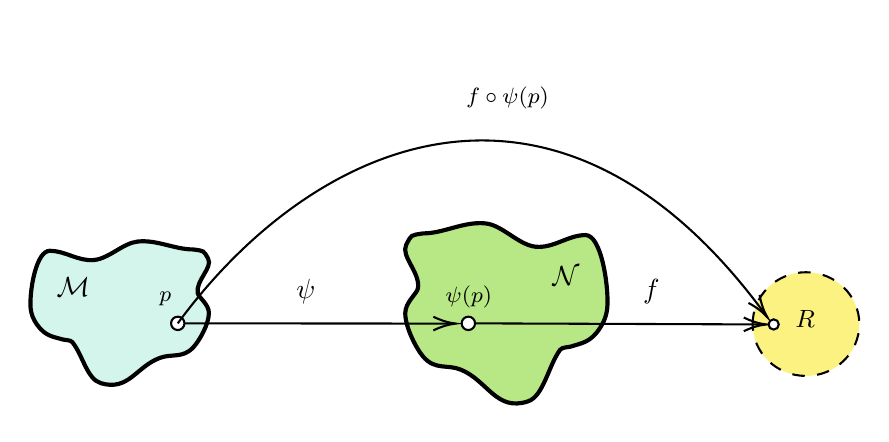
\begin{tikzpicture}[x=0.75pt,y=0.75pt,yscale=-1,xscale=1]
%uncomment if require: \path (0,230); %set diagram left start at 0, and has height of 230

%Shape: Boxed Bezier Curve [id:dp548963754265211] 
\draw [fill={rgb, 255:red, 211; green, 245; blue, 236 }  ,fill opacity=1 ][line width=1.5]    (171.39,104.78) .. controls (162.43,104.78) and (154.14,100.07) .. (144.78,100.95) .. controls (137.56,101.64) and (130.84,109.2) .. (123.56,109.88) .. controls (116,110.59) and (109.74,105.42) .. (102.34,105.42) .. controls (95.72,105.42) and (92.63,123.97) .. (92.99,132.2) .. controls (93.16,136.07) and (94.49,138.74) .. (96.23,141.13) .. controls (100.21,146.62) and (103.87,146.79) .. (108.45,148.14) .. controls (109.52,148.46) and (112.26,148.35) .. (113.13,149.42) .. controls (118.12,155.54) and (120.17,167.23) .. (126.8,169.19) .. controls (140.3,173.18) and (143.75,161.42) .. (155.21,157.07) .. controls (161.15,154.81) and (166.24,157.45) .. (171.39,151.97) .. controls (174.16,149.02) and (178.94,140.93) .. (178.94,135.39) .. controls (178.94,131.1) and (173.94,127.93) .. (173.55,125.82) .. controls (172.44,119.91) and (180.95,113.45) .. (178.58,109.24) .. controls (176.26,105.12) and (176.78,105.56) .. (171.39,104.78) -- cycle ;
%Shape: Ellipse [id:dp29255012486968357] 
\draw  [fill={rgb, 255:red, 248; green, 231; blue, 28 }  ,fill opacity=0.55 ][dash pattern={on 4.5pt off 4.5pt}] (440.91,140.74) .. controls (440.91,126.94) and (452.42,115.76) .. (466.62,115.76) .. controls (480.81,115.76) and (492.32,126.94) .. (492.32,140.74) .. controls (492.32,154.54) and (480.81,165.72) .. (466.62,165.72) .. controls (452.42,165.72) and (440.91,154.54) .. (440.91,140.74) -- cycle ;
%Shape: Boxed Bezier Curve [id:dp2261869946937909] 
\draw [fill={rgb, 255:red, 126; green, 211; blue, 33 }  ,fill opacity=0.55 ][line width=1.5]    (282.11,97.05) .. controls (292.27,97.05) and (301.66,91.12) .. (312.27,92.24) .. controls (320.45,93.1) and (328.07,102.61) .. (336.32,103.46) .. controls (344.89,104.35) and (351.99,97.85) .. (360.37,97.85) .. controls (367.88,97.85) and (371.37,121.16) .. (370.97,131.5) .. controls (370.78,136.36) and (369.27,139.71) .. (367.3,142.72) .. controls (362.78,149.63) and (358.64,149.83) .. (353.44,151.54) .. controls (352.24,151.93) and (349.13,151.8) .. (348.14,153.14) .. controls (342.49,160.84) and (340.17,175.52) .. (332.65,177.98) .. controls (317.35,182.99) and (313.44,168.22) .. (300.45,162.75) .. controls (293.72,159.92) and (287.94,163.23) .. (282.11,156.34) .. controls (278.97,152.64) and (273.55,142.47) .. (273.55,135.51) .. controls (273.55,130.12) and (279.21,126.14) .. (279.66,123.49) .. controls (280.92,116.06) and (271.27,107.94) .. (273.96,102.66) .. controls (276.59,97.48) and (275.99,98.02) .. (282.11,97.05) -- cycle ;
%Straight Lines [id:da573620974924035] 
\draw    (163.94,140.39) -- (296,140.5) ;
\draw [shift={(298,140.5)}, rotate = 180.05] [color={rgb, 255:red, 0; green, 0; blue, 0 }  ][line width=0.75]    (10.93,-3.29) .. controls (6.95,-1.4) and (3.31,-0.3) .. (0,0) .. controls (3.31,0.3) and (6.95,1.4) .. (10.93,3.29)   ;
%Straight Lines [id:da00667541340455724] 
\draw    (307.17,140.39) -- (445.58,140.91) ;
\draw [shift={(447.58,140.92)}, rotate = 180.22] [color={rgb, 255:red, 0; green, 0; blue, 0 }  ][line width=0.75]    (10.93,-3.29) .. controls (6.95,-1.4) and (3.31,-0.3) .. (0,0) .. controls (3.31,0.3) and (6.95,1.4) .. (10.93,3.29)   ;
%Shape: Circle [id:dp8370900540926526] 
\draw  [fill={rgb, 255:red, 255; green, 255; blue, 255 }  ,fill opacity=1 ] (160.72,140.39) .. controls (160.72,138.61) and (162.16,137.16) .. (163.94,137.16) .. controls (165.72,137.16) and (167.17,138.61) .. (167.17,140.39) .. controls (167.17,142.17) and (165.72,143.61) .. (163.94,143.61) .. controls (162.16,143.61) and (160.72,142.17) .. (160.72,140.39) -- cycle ;
%Shape: Circle [id:dp1381101300882457] 
\draw  [fill={rgb, 255:red, 255; green, 255; blue, 255 }  ,fill opacity=1 ] (300.72,140.39) .. controls (300.72,138.61) and (302.16,137.16) .. (303.94,137.16) .. controls (305.72,137.16) and (307.17,138.61) .. (307.17,140.39) .. controls (307.17,142.17) and (305.72,143.61) .. (303.94,143.61) .. controls (302.16,143.61) and (300.72,142.17) .. (300.72,140.39) -- cycle ;
%Curve Lines [id:da7070782507909167] 
\draw    (163.94,140.39) .. controls (229,51.7) and (347,-1.57) .. (448,137.45) ;
\draw [shift={(448,137.45)}, rotate = 234] [color={rgb, 255:red, 0; green, 0; blue, 0 }  ][line width=0.75]    (10.93,-3.29) .. controls (6.95,-1.4) and (3.31,-0.3) .. (0,0) .. controls (3.31,0.3) and (6.95,1.4) .. (10.93,3.29)   ;
%Shape: Circle [id:dp9897406803094917] 
\draw  [fill={rgb, 255:red, 255; green, 255; blue, 255 }  ,fill opacity=1 ] (453.52,140.92) .. controls (453.52,139.55) and (452.41,138.45) .. (451.05,138.45) .. controls (449.69,138.45) and (448.58,139.55) .. (448.58,140.92) .. controls (448.58,142.28) and (449.69,143.38) .. (451.05,143.38) .. controls (452.41,143.38) and (453.52,142.28) .. (453.52,140.92) -- cycle ;

% Text Node
\draw (104.02,116.65) node [anchor=north west][inner sep=0.75pt]  [font=\normalsize]  {$\mathcal{M}$};
% Text Node
\draw (219.61,117.78) node [anchor=north west][inner sep=0.75pt]    {$\psi $};
% Text Node
\draw (343.02,111.65) node [anchor=north west][inner sep=0.75pt]  [font=\normalsize]  {$\mathcal{N}$};
% Text Node
\draw (386.61,117.78) node [anchor=north west][inner sep=0.75pt]    {$f$};
% Text Node
\draw (460.02,132.65) node [anchor=north west][inner sep=0.75pt]  [font=\small]  {$\mathbb{R}$};
% Text Node
\draw (153.55,123.85) node [anchor=north west][inner sep=0.75pt]  [font=\footnotesize]  {$p$};
% Text Node
\draw (291.55,120.85) node [anchor=north west][inner sep=0.75pt]  [font=\footnotesize]  {$\psi ( p)$};
% Text Node
\draw (301.55,24.85) node [anchor=north west][inner sep=0.75pt]  [font=\footnotesize]  {$f\circ \psi ( p)$};


\end{tikzpicture}
